% !TEX program = xelatex
% Build: xelatex -shell-escape main.tex  (twice)
\documentclass[10.5pt,a4paper]{article}

\usepackage[a4paper,left=2.3cm,right=2.3cm,top=2.5cm,bottom=2.5cm]{geometry}
\usepackage{fontspec}
\setmainfont{Latin Modern Roman}[Ligatures=TeX]
\setsansfont{Latin Modern Sans}[Ligatures=TeX]
\setmonofont{DejaVu Sans Mono}[Scale=MatchLowercase]
\newfontfamily\symfont{DejaVu Sans}
\usepackage{unicode-math}
\setmathfont{Latin Modern Math}

\usepackage[table]{xcolor}
\definecolor{accent}{HTML}{1F4E79}
\definecolor{accent2}{HTML}{B45309}
\definecolor{okgreen}{HTML}{15803D}
\definecolor{badred}{HTML}{B91C1C}
\definecolor{codebg}{HTML}{F6F8FA}
\definecolor{errbg}{HTML}{FDF2F2}
\definecolor{softgray}{HTML}{6B7280}

\usepackage{booktabs,longtable,array}
\usepackage{enumitem}
\setlist{itemsep=2pt,topsep=4pt,parsep=0pt}
\usepackage{needspace}
\usepackage{fancyhdr}
\usepackage{titlesec}
\usepackage[most]{tcolorbox}
\usepackage{tikz}
\usetikzlibrary{arrows.meta,positioning,calc,fit,backgrounds}

% ---------- minted ----------
\usepackage{minted}
\setminted{style=friendly,fontsize=\footnotesize,bgcolor=codebg,frame=leftline,
  framerule=2.2pt,rulecolor=accent,framesep=7pt,breaklines,baselinestretch=1.05}
\newmintinline[rs]{rust}{bgcolor={},fontsize=\normalsize}

% code-in-arguments helpers (verbatim is not allowed in macro arguments)
\newcommand{\st}{\texorpdfstring{\texttt{\textquotesingle static}}{'static}}
\newcommand{\us}{\texorpdfstring{\texttt{\textquotesingle\_}}{'\_}}
\newcommand{\ta}{\texorpdfstring{\texttt{\textquotesingle a}}{'a}}
\newcommand{\Tst}{\texorpdfstring{\texttt{T: \textquotesingle static}}{T: 'static}}
\newcommand{\refst}{\texorpdfstring{\texttt{\&\textquotesingle static}}{\&'static}}

\expandafter\gdef\csname nl@c@fail_01_dangling\endcsname{13}
\expandafter\gdef\csname nl@e@fail_01_dangling\endcsname{11}
\expandafter\gdef\csname nl@c@ok_21_lookup_explicit\endcsname{18}
\expandafter\gdef\csname nl@r@ok_21_lookup_explicit\endcsname{1}
\expandafter\gdef\csname nl@c@ok_10_object_defaults\endcsname{30}
\expandafter\gdef\csname nl@r@ok_10_object_defaults\endcsname{1}
\expandafter\gdef\csname nl@c@ok_19_struct_fixes\endcsname{28}
\expandafter\gdef\csname nl@r@ok_19_struct_fixes\endcsname{1}
\expandafter\gdef\csname nl@c@ok_07_static_sources\endcsname{15}
\expandafter\gdef\csname nl@r@ok_07_static_sources\endcsname{1}
\expandafter\gdef\csname nl@c@fail_11_error_box\endcsname{9}
\expandafter\gdef\csname abr@fail_11_error_box\endcsname{}
\expandafter\gdef\csname nl@e@fail_11_error_box\endcsname{16}
\expandafter\gdef\csname nl@c@ok_12_hrtb\endcsname{20}
\expandafter\gdef\csname nl@r@ok_12_hrtb\endcsname{2}
\expandafter\gdef\csname nl@c@fail_20_static_field_local\endcsname{10}
\expandafter\gdef\csname nl@e@fail_20_static_field_local\endcsname{13}
\expandafter\gdef\csname nl@c@ok_23_contract_v1\endcsname{15}
\expandafter\gdef\csname nl@r@ok_23_contract_v1\endcsname{1}
\expandafter\gdef\csname nl@c@fail_10_boxed_static\endcsname{10}
\expandafter\gdef\csname abr@fail_10_boxed_static\endcsname{}
\expandafter\gdef\csname nl@e@fail_10_boxed_static\endcsname{12}
\expandafter\gdef\csname nl@c@ok_08_static_bound\endcsname{19}
\expandafter\gdef\csname nl@r@ok_08_static_bound\endcsname{6}
\expandafter\gdef\csname nl@c@ok_14_E0310_fixed\endcsname{9}
\expandafter\gdef\csname nl@r@ok_14_E0310_fixed\endcsname{1}
\expandafter\gdef\csname nl@c@fail_17_cell_invariance\endcsname{8}
\expandafter\gdef\csname nl@e@fail_17_cell_invariance\endcsname{12}
\expandafter\gdef\csname nl@c@fail_23_contract_v2\endcsname{15}
\expandafter\gdef\csname nl@e@fail_23_contract_v2\endcsname{11}
\expandafter\gdef\csname nl@c@fail_21_rule_first\endcsname{6}
\expandafter\gdef\csname abr@fail_21_rule_first\endcsname{}
\expandafter\gdef\csname nl@e@fail_21_rule_first\endcsname{27}
\expandafter\gdef\csname nl@c@ok_13_covariance\endcsname{10}
\expandafter\gdef\csname nl@r@ok_13_covariance\endcsname{1}
\expandafter\gdef\csname nl@c@fail_09_spawn_borrow\endcsname{7}
\expandafter\gdef\csname nl@e@fail_09_spawn_borrow\endcsname{17}
\expandafter\gdef\csname nl@c@fail_16_struct_field_elided\endcsname{4}
\expandafter\gdef\csname nl@c@ok_02_nll\endcsname{7}
\expandafter\gdef\csname nl@r@ok_02_nll\endcsname{2}
\expandafter\gdef\csname nl@c@ok_18_elision_fixes\endcsname{28}
\expandafter\gdef\csname nl@r@ok_18_elision_fixes\endcsname{3}
\expandafter\gdef\csname nl@c@fail_02_nll\endcsname{6}
\expandafter\gdef\csname nl@e@fail_02_nll\endcsname{9}
\expandafter\gdef\csname nl@c@fail_19_struct_single_ref\endcsname{6}
\expandafter\gdef\csname nl@e@fail_19_struct_single_ref\endcsname{11}
\expandafter\gdef\csname nl@c@ok_09_threads\endcsname{16}
\expandafter\gdef\csname nl@r@ok_09_threads\endcsname{4}
\expandafter\gdef\csname nl@c@fail_24_trait_no_body\endcsname{6}
\expandafter\gdef\csname nl@e@fail_24_trait_no_body\endcsname{11}
\expandafter\gdef\csname nl@c@fail_18_elision_cases\endcsname{11}
\expandafter\gdef\csname nl@e@fail_18_elision_cases\endcsname{23}
\expandafter\gdef\csname nl@c@fail_04_ambiguous\endcsname{6}
\expandafter\gdef\csname nl@e@fail_04_ambiguous\endcsname{23}
\expandafter\gdef\csname nl@c@fail_06_rpit\endcsname{9}
\expandafter\gdef\csname nl@e@fail_06_rpit\endcsname{14}
\expandafter\gdef\csname nl@c@fail_13_invariance\endcsname{12}
\expandafter\gdef\csname nl@e@fail_13_invariance\endcsname{12}
\expandafter\gdef\csname nl@c@ok_03_parser\endcsname{44}
\expandafter\gdef\csname nl@r@ok_03_parser\endcsname{1}
\expandafter\gdef\csname nl@c@ok_05_dyn_underscore\endcsname{9}
\expandafter\gdef\csname nl@r@ok_05_dyn_underscore\endcsname{1}
\expandafter\gdef\csname nl@c@fail_14_E0310\endcsname{9}
\expandafter\gdef\csname nl@e@fail_14_E0310\endcsname{13}
\expandafter\gdef\csname nl@c@fail_03_elided_self\endcsname{21}
\expandafter\gdef\csname abr@fail_03_elided_self\endcsname{}
\expandafter\gdef\csname nl@e@fail_03_elided_self\endcsname{9}
\expandafter\gdef\csname nl@c@ok_11_error_box\endcsname{28}
\expandafter\gdef\csname nl@r@ok_11_error_box\endcsname{1}
\expandafter\gdef\csname nl@c@fail_22_rule_unify\endcsname{6}
\expandafter\gdef\csname abr@fail_22_rule_unify\endcsname{}
\expandafter\gdef\csname nl@e@fail_22_rule_unify\endcsname{11}
\expandafter\gdef\csname nl@c@ok_04_underscore_return\endcsname{17}
\expandafter\gdef\csname nl@e@ok_04_underscore_return\endcsname{15}
\expandafter\gdef\csname nl@r@ok_04_underscore_return\endcsname{1}
\expandafter\gdef\csname nl@c@ok_06_rpit\endcsname{8}
\expandafter\gdef\csname nl@r@ok_06_rpit\endcsname{1}
\expandafter\gdef\csname nl@c@ok_17_box_covariance\endcsname{7}
\expandafter\gdef\csname nl@r@ok_17_box_covariance\endcsname{1}
\expandafter\gdef\csname nl@c@ok_01_longest\endcsname{13}
\expandafter\gdef\csname nl@r@ok_01_longest\endcsname{1}
\expandafter\gdef\csname nl@c@fail_05_dyn_static\endcsname{9}
\expandafter\gdef\csname nl@e@fail_05_dyn_static\endcsname{12}
\expandafter\gdef\csname nl@c@fail_08_static_bound\endcsname{6}
\expandafter\gdef\csname nl@e@fail_08_static_bound\endcsname{12}
\expandafter\gdef\csname nl@c@ok_15_static_table\endcsname{18}
\expandafter\gdef\csname nl@r@ok_15_static_table\endcsname{1}
\expandafter\gdef\csname nl@c@fail_15_static_table_no\endcsname{10}

\newdimen\tmpd
\newcommand{\needlines}[2]{\tmpd=\dimexpr#2*(#1)\relax
  \ifdim\tmpd>0.8\textheight\tmpd=0.8\textheight\fi\needspace{\tmpd}}
\newcounter{lst}
\newcommand{\lsthead}[3]{%
  \needlines{\csname nl@c@#2\endcsname+4}{12pt}%
  \refstepcounter{lst}\par\addvspace{7pt}\noindent
  {\sffamily\small\bfseries Listing~\thelst}\hspace{0.6em}{\sffamily\small #3}\hfill
  \ifx#1o{\colorbox{okgreen!14}{\sffamily\scriptsize\color{okgreen}{\symfont ✓}\,compiles}}\fi
  \ifx#1f{\colorbox{badred!12}{\sffamily\scriptsize\color{badred}{\symfont ✗}\,rejected}}\fi
  \par\nopagebreak\vspace{-2pt}%
  {\ttfamily\scriptsize\color{softgray}\detokenize{#2}.rs}%
  \ifcsname abr@#2\endcsname{\sffamily\scriptsize\color{softgray}\ (abridged)}\fi
  \par\nopagebreak\vspace{-8pt}}
\newcommand{\codefile}[1]{\IfFileExists{lst/#1.rs}{\inputminted{rust}{lst/#1.rs}}{\inputminted{rust}{ex/#1.rs}}}
% \ok{file}{caption} / \fail{file}{caption}
\newcommand{\ok}[2]{\lsthead{o}{#1}{#2}\codefile{#1}}
\newcommand{\fail}[2]{\lsthead{f}{#1}{#2}\codefile{#1}}
% compiler output / program output excerpts
\newcommand{\diag}[1]{\needlines{\csname nl@e@#1\endcsname+2}{10pt}\par\vspace{-13pt}\inputminted[fontsize=\scriptsize,bgcolor=errbg,rulecolor=badred!70]{text}{out/#1.excerpt}\par\vspace{2pt}}
\newcommand{\runout}[1]{\needlines{\csname nl@r@#1\endcsname+2}{10pt}\par\vspace{-13pt}\inputminted[fontsize=\scriptsize,bgcolor=okgreen!7,rulecolor=okgreen!70]{text}{out/#1.run}\par\vspace{2pt}}

% ---------- boxes ----------
\newtcolorbox{keyidea}[1][Key idea]{enhanced,breakable,colback=accent!5,colframe=accent,
  fonttitle=\sffamily\bfseries\small,title={#1},boxrule=0.5pt,arc=2pt,
  left=6pt,right=6pt,top=3pt,bottom=3pt,before skip=8pt,after skip=8pt}
\newtcolorbox{pitfall}[1][Pitfall]{enhanced,breakable,colback=accent2!6,colframe=accent2,
  fonttitle=\sffamily\bfseries\small,title={#1},boxrule=0.5pt,arc=2pt,
  left=6pt,right=6pt,top=3pt,bottom=3pt,before skip=8pt,after skip=8pt}

% ---------- headings / page style ----------
\titleformat{\section}{\sffamily\bfseries\Large\color{accent}}{\thesection}{0.7em}{}
\titleformat{\subsection}{\sffamily\bfseries\large\color{accent}}{\thesubsection}{0.7em}{}
\titleformat{\subsubsection}{\sffamily\bfseries\normalsize}{\thesubsubsection}{0.7em}{}
\titlespacing*{\section}{0pt}{20pt}{8pt}
\titlespacing*{\subsection}{0pt}{14pt}{5pt}
\pagestyle{fancy}\fancyhf{}
\fancyhead[L]{\sffamily\small\color{softgray}Rust Lifetimes --- a field guide}
\fancyhead[R]{\sffamily\small\color{softgray}\leftmark}
\fancyfoot[C]{\sffamily\small\thepage}
\renewcommand{\headrulewidth}{0.3pt}
\renewcommand{\sectionmark}[1]{\markboth{#1}{}}
\setlength{\parindent}{0pt}\setlength{\parskip}{5pt}
\let\origsubsection\subsection
\renewcommand{\subsection}{\needspace{7\baselineskip}\origsubsection}
\let\origsection\section
\renewcommand{\section}{\needspace{9\baselineskip}\origsection}
\renewcommand{\arraystretch}{1.25}
\setlength{\emergencystretch}{2em}

\usepackage[colorlinks=true,linkcolor=accent,urlcolor=accent,citecolor=accent,
  pdftitle={Rust Lifetimes: a field guide},pdfauthor={},
  pdfsubject={Lifetimes, the anonymous lifetime and static in Rust}]{hyperref}

\fancypagestyle{plain}{\fancyhf{}\fancyfoot[C]{\sffamily\small\thepage}\renewcommand{\headrulewidth}{0pt}}
\begin{document}
\thispagestyle{plain}

% ================= TITLE BLOCK =================
\begin{tcolorbox}[enhanced,colback=accent,colframe=accent,coltext=white,arc=3pt,
  left=14pt,right=14pt,top=12pt,bottom=12pt]
{\sffamily\bfseries\fontsize{26}{30}\selectfont Rust Lifetimes}\\[4pt]
{\sffamily\large A field guide to regions, elision and variance ---\\
with a close reading of \texttt{\textquotesingle\_} and \texttt{\textquotesingle static}}\\[8pt]
{\sffamily\small Every program in this document was compiled with \texttt{rustc 1.75.0}, edition~2021.
Compiler diagnostics are quoted verbatim; passing and failing examples are marked.}
\end{tcolorbox}

\begin{keyidea}[In one page]
\begin{itemize}
\item A lifetime is a \emph{compile-time region} (a set of program points), never a runtime value. Annotations
  \emph{describe} relationships between borrows; they cannot make anything live longer.
\item \us\ is not a lifetime name. It means ``some lifetime I don't need to name'': fresh for each parameter,
  resolved by the elision rules in a return type, and inferred in a body. Its three real jobs are (i) exposing
  hidden lifetime parameters, (ii) \rs{impl}-headers, and (iii) opting trait objects and \rs{impl Trait} into
  borrowing (\rs{dyn Trait + '_}).
\item \st\ has \emph{two} meanings: \rs{&'static T} (a reference valid for the rest of the program) and
  \rs{T: 'static} (a \emph{bound}: ``$T$ holds no borrow that can expire''). The bound is far more common,
  and it does \textbf{not} mean the value lives forever: a local \rs{String} is \rs{'static}.
\item Default trait-object bounds are the hidden source of most \st\ errors: \rs{Box<dyn Trait>} means
  \rs{Box<dyn Trait + 'static>}, whereas \rs{&'a dyn Trait} means \rs{&'a (dyn Trait + 'a)}.
\end{itemize}
\end{keyidea}

\setcounter{tocdepth}{1}
\tableofcontents

% ================= 1 =================
\section{The mental model: regions, not durations}

For the borrow checker, a lifetime \rs{'a} is a \emph{region}: a set of points in the control-flow graph of a function
body. A reference \rs{&'a T} is a promise that the referent stays valid, and is not accessed in a conflicting way,
at every point of \rs{'a}. Three consequences shape everything else in this guide.

\begin{enumerate}
\item \textbf{Lifetimes are erased.} They have no runtime representation and do not influence code generation;
  they exist only to give the checker a system of constraints to solve.
\item \textbf{They follow use, not scope.} Since non-lexical lifetimes (NLL), a borrow is live from its creation up
  to the last point where a reference derived from it \emph{may still be used}, not to the closing brace of the
  enclosing block.
\item \textbf{Only signatures carry lifetimes you write.} Inside a body the compiler infers every region on its own;
  at function boundaries, annotations (or their elided defaults) are the contract.
\end{enumerate}

\begin{figure}[h]
\centering
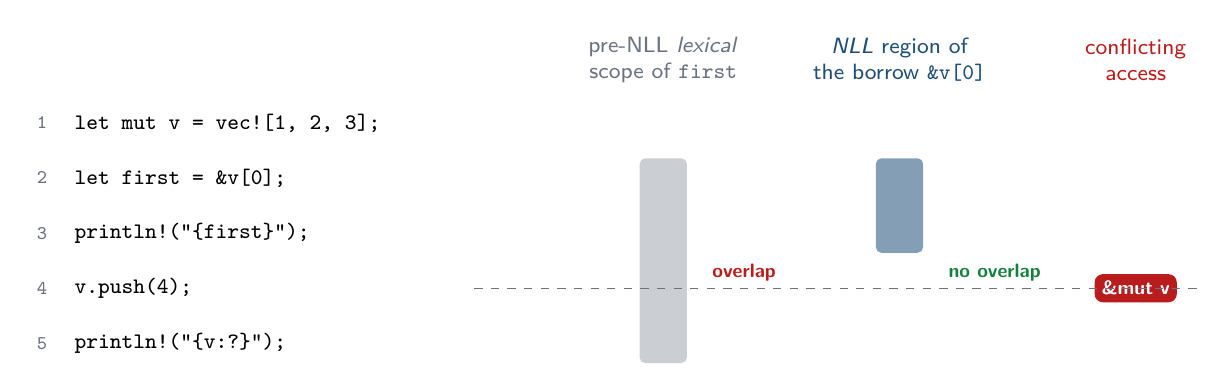
\begin{tikzpicture}[font=\sffamily\footnotesize,x=1cm,y=1cm,
  cl/.style={font=\ttfamily\footnotesize,anchor=west},
  num/.style={font=\ttfamily\scriptsize,text=softgray,anchor=east}]
  % code
  \foreach \i/\cc in {1/{let mut v = vec![1, 2, 3];},2/{let first = \&v[0];},3/{println!("\{first\}");},4/{v.push(4);},5/{println!("\{v:?\}");}} {
    \node[num] at (-0.1,-\i*0.7) {\i};
    \node[cl] at (0,-\i*0.7) {\cc};
  }
  % column headers
  \node[align=center,text=softgray] at (7.6,0.1) {pre-NLL \emph{lexical}\\ scope of \texttt{first}};
  \node[align=center,text=accent] at (10.6,0.1) {\emph{NLL} region of\\ the borrow \texttt{\&v[0]}};
  \node[align=center,text=badred] at (13.6,0.1) {conflicting\\ access};
  % lexical bar
  \fill[softgray!35,rounded corners=2pt] (7.3,-2*0.7+0.25) rectangle (7.9,-5*0.7-0.25);
  % NLL bar
  \fill[accent!55,rounded corners=2pt] (10.3,-2*0.7+0.25) rectangle (10.9,-3*0.7-0.25);
  % conflict marker
  \node[fill=badred,text=white,rounded corners=3pt,inner sep=2.5pt,font=\sffamily\bfseries\scriptsize] at (13.6,-4*0.7) {\&mut v};
  % guides at line 4
  \draw[dashed,softgray] (5.2,-4*0.7) -- (14.4,-4*0.7);
  \node[text=badred,font=\sffamily\bfseries\scriptsize,anchor=west] at (8.1,-4*0.7+0.2) {overlap};
  \node[text=okgreen,font=\sffamily\bfseries\scriptsize,anchor=west] at (11.1,-4*0.7+0.2) {no overlap};
\end{tikzpicture}
\caption{Why Listing~\ref{lst:nllok} compiles. The borrow \texttt{\&v[0]} is live only until its last use (line~3), so the
\texttt{v.push} on line~4 does not intersect it. A purely lexical rule would keep it alive to the end of the block.}
\end{figure}

\ok{ok_02_nll}{NLL: the borrow ends at its last use}\label{lst:nllok}
\runout{ok_02_nll}
\fail{fail_02_nll}{Move the later use after the \texttt{push} and the borrow is live across it}
\diag{fail_02_nll}

\subsection{Annotations describe; they never extend}

\ok{ok_01_longest}{The classic \texttt{longest}}

In \rs{fn longest<'a>(x: &'a str, y: &'a str) -> &'a str} the single name \ta\ says: ``the result is valid only where
\emph{both} inputs are'', i.e.\ for the intersection of their regions. The body is checked against this signature
(returning \rs{x} or \rs{y} is justified), and every caller is checked against it \emph{and nothing else}. This
modularity is why the defaults chosen by elision (Section~\ref{sec:elision}) matter so much: they \emph{are} the contract.

\fail{fail_01_dangling}{Use the result after one input died}
\diag{fail_01_dangling}

Here \ta\ must cover the final \rs{println!}, because \rs{result} is used there; but \rs{&inner} is valid only inside the
inner block. Nothing in the \emph{body} of \rs{longest} is wrong; the contradiction is between the call site and the
contract.

\subsection{Notation}

\begin{longtable}{@{}p{3.1cm}p{3.6cm}p{8.7cm}@{}}
\toprule
\textbf{Syntax} & \textbf{Read as} & \textbf{Meaning}\\\midrule\endhead
\rs{'a} & ``lifetime a'' & A region variable.\\
\rs{&'a T} & & Reference to a \rs{T}, valid throughout \rs{'a}.\\
\rs{'a: 'b} & ``\rs{'a} outlives \rs{'b}'' & Region \rs{'a} contains every point of \rs{'b}.\\
\rs{T: 'a} & ``\rs{T} outlives \rs{'a}'' & Every lifetime occurring inside \rs{T} outlives \rs{'a}: values of type \rs{T} stay valid throughout \rs{'a}.\\
\rs{'static} & & The region covering the whole program; it outlives every other lifetime.\\
\rs{'_} & ``anonymous lifetime'' & Placeholder; see Section~\ref{sec:underscore}.\\
\rs{for<'a> ...} & ``for all \rs{'a}'' & Higher-ranked quantification; see Section~\ref{sec:hrtb}.\\
\bottomrule
\end{longtable}

Writing \rs{&'a T} also \emph{implies} \rs{T: 'a} (the type must be well-formed); this is why you almost never write that bound by hand.

% ================= 2 =================
\section{Types and methods: whose borrow is it?}
\label{sec:whose}

A struct that stores a reference needs a lifetime parameter, and that parameter is part of the type: \rs{Parser<'x>} and
\rs{Parser<'y>} are different types, related by variance (Section~\ref{sec:variance}). Inside \rs{impl<'src> Parser<'src>},
the name \rs{'src} denotes the lifetime of the \emph{data the parser reads}. Every method additionally gets its own
anonymous lifetime for \rs{&self} or \rs{&mut self}. A method returning a reference therefore has a genuine choice:

\begin{center}
\begin{tabular}{@{}lll@{}}
\toprule
\textbf{Return type} & \textbf{Result borrows from} & \textbf{Effect on the caller}\\\midrule
\rs{Option<&'src str>} & the \emph{text} & parser is free again; results can be kept across calls\\
\rs{Option<&str>} (elided) & the \emph{\rs{&mut self} borrow} & parser stays exclusively borrowed while any result lives\\
\bottomrule
\end{tabular}
\end{center}

Elision always picks the second row (rule~3, Section~\ref{sec:elision}). That is correct for something like
\rs{fn buf(&mut self) -> &mut [u8]}, but wrong for tokenisers, iterators and cursors:

\ok{ok_03_parser}{Returning \texttt{\textquotesingle src} instead of the \texttt{\&mut self} lifetime}\label{lst:parsersrc}
\runout{ok_03_parser}
\fail{fail_03_elided_self}{Same code, elided return type: results pin the parser}
\diag{fail_03_elided_self}

\begin{keyidea}[Rule of thumb]
If the reference you return points into data that the struct merely \emph{holds a reference to}, name the struct's own
lifetime in the return type. This is exactly why \rs{slice::Iter<'a, T>::next} can return \rs{Option<&'a T>} and you can
collect many items while the iterator is still in use. A ``lending'' iterator, whose items \emph{do} borrow from
\rs{&mut self}, cannot be expressed by \rs{Iterator} at all.
\end{keyidea}

% ================= 3 =================
\section{Lifetime elision}
\label{sec:elision}

Elision is a fixed, purely syntactic rewrite applied to function signatures (and to \rs{Fn(..)} sugar and \rs{impl}
headers). It never looks at the body.

\begin{enumerate}
\item Each elided lifetime in the \emph{inputs} becomes a distinct fresh lifetime parameter.
\item If there is \emph{exactly one} input lifetime position (elided or named), that lifetime is assigned to all elided output lifetimes.
\item If there are several, but one of them is \rs{&self} or \rs{&mut self}, the lifetime of \rs{self} is assigned to all elided output lifetimes.
\end{enumerate}
Otherwise elision fails with E0106 (``missing lifetime specifier'').
\needspace{16\baselineskip}

\begin{longtable}{@{}p{5.7cm}p{6.2cm}p{3.5cm}@{}}
\toprule
\textbf{You write} & \textbf{The compiler reads} & \textbf{Rule}\\\midrule\endhead
\rs{fn f(x: &str) -> &str} & \rs{fn f<'a>(x: &'a str) -> &'a str} & 1, 2\\
\rs{fn f(x: &str, y: &str) -> &str} & \emph{error E0106} & 1, none applies\\
\rs{fn f<'a>(x: &'a str, y: &str) -> &str} & \emph{error E0106} (two input lifetimes) & none applies\\
\rs{fn m(&self, k: &str) -> &str} & \rs{fn m<'s,'k>(&'s self, k: &'k str) -> &'s str} & 1, 3\\
\rs{fn f(x: &mut &str)} & \rs{fn f<'a,'b>(x: &'a mut &'b str)} (independent) & 1\\
\rs{fn f(s: &str) -> Iter} & \rs{fn f<'a>(s: &'a str) -> Iter<'a>} (hidden; prefer \rs{Iter<'_>}) & 1, 2\\
\rs{fn(&str) -> &str} (pointer type) & \rs{for<'a> fn(&'a str) -> &'a str} & HR, 1, 2\\
\rs{static S: &str} / \rs{const C: &[u8]} & \rs{&'static str} / \rs{&'static [u8]} & item default\\
\bottomrule
\end{longtable}

\subsection{Why those two rows are errors}
\label{sec:e0106}

Take the two rejected signatures from the table and apply the rules mechanically.

\textbf{Case A:} \rs{fn f(x: &str, y: &str) -> &str}.
\begin{enumerate}[label=\arabic*.]
\item Rule~1 gives each elided \emph{input} its own fresh lifetime: \rs{fn f<'1, '2>(x: &'1 str, y: &'2 str) -> &'? str}.
\item Rule~2 applies only if there is \emph{exactly one} input lifetime. There are two, so it is skipped.
\item Rule~3 applies only if one input is \rs{&self} or \rs{&mut self}. Neither is, so it is skipped.
\end{enumerate}
No rule fills in \rs{'?}, so elision fails with E0106.

\textbf{Case B:} \rs{fn f<'a>(x: &'a str, y: &str) -> &str}.
Rule~2 counts \emph{every} lifetime position in the inputs, named or elided. Here there are two: the named \ta\ and a fresh
anonymous one for \rs{y}. The count is therefore two, rule~2 is skipped, there is no \rs{self}, and again nothing
determines the output. Naming one input does not make it ``the'' input; the compiler does not guess that the named one,
or the elided one, is the intended source.

\textbf{No further rule can rescue these cases.} Elision is a closed set of exactly the three rules above; the compiler
does not fall back to a heuristic when they run out. It will not pick ``the first parameter'', ``the longest-lived
input'', ``the named one'' or ``whichever the body returns'', and writing \us\ in the output does not help either, because
\us\ in a return type just \emph{requests} elision (Listing~\ref{lst:ambig}). Once rules~2 and~3 both fail, the only way
forward is to write the output lifetime explicitly. Section~\ref{sec:badrules} tests the most natural candidate rules and shows concretely how each one fails.

\ok{ok_18_elision_fixes}{Three honest ways to state the contract}
\runout{ok_18_elision_fixes}
\fail{fail_18_elision_cases}{Cases A and B from the table}
\diag{fail_18_elision_cases}

\begin{keyidea}[Why the compiler refuses to guess]
The compiler never inspects the body to resolve elision. In case~A the body happens to return either \rs{x} or
\rs{y}, and in case~B only \rs{x}, but the signature is the \emph{contract} that callers are checked against. If the
body could silently change the contract, editing the body (say, returning \rs{y} instead of \rs{x}) would break callers
in other crates without touching the signature. Requiring you to write the relationship keeps the signature
authoritative, and the compiler's own hint above spells out the question it cannot answer: ``borrowed from \rs{x} or
\rs{y}?''
\end{keyidea}

The choice is a real design decision, not a syntax chore:

\begin{center}
\begin{tabular}{@{}p{5.4cm}p{4.2cm}p{5.4cm}@{}}
\toprule
\textbf{Signature} & \textbf{Result may borrow from} & \textbf{Caller consequence}\\\midrule
\rs{fn f<'a>(x: &'a str, y: &'a str) -> &'a str} & either input & result must not outlive \emph{either} argument\\
\rs{fn f<'a>(x: &'a str, y: &str) -> &'a str} & only \rs{x} & \rs{y} may die while the result lives; the body may not return \rs{y}\\
\rs{fn f(x: &str, y: &str) -> String} & neither & no borrow at all\\
\bottomrule
\end{tabular}
\end{center}

\subsection{Why a single reference in a struct cannot be elided}
\label{sec:structelide}

Strip the problem to its minimum: one struct, one field, one reference. If elision ever worked for a type, it would work here.

\fail{fail_19_struct_single_ref}{The simplest struct with a reference}
\diag{fail_19_struct_single_ref}

The error is E0106 even though there is only one reference and nothing to be ambiguous about. Writing \rs{&'_ str} gives
E0106 and writing \rs{&'a str} without declaring \rs{'a} gives E0261 (both verified in Appendix~A, \texttt{fail\_16}). The reasons are structural, not a
matter of missing rules.

\begin{enumerate}[label=\arabic*.]
\item \textbf{Elision is defined over function signatures.} Its rules choose the output lifetimes from the \emph{input}
  lifetimes. A struct definition has no inputs and no outputs: a field is not a parameter, so ``exactly one input lifetime''
  (rule~2) has nothing to count. The fact that there is a single reference is irrelevant.
\item \textbf{In a struct the lifetime is part of the type, so it must be declared.} A function's fresh lifetimes
  (rule~1) are local to its signature and change nothing outside it. A struct field's lifetime would have to become a
  parameter of the struct itself: \rs{Holder} would secretly be \rs{Holder<'x>}. Every use of the type, every \rs{impl},
  every field of another struct, and the variance computation (Section~\ref{sec:variance}) depend on that parameter, yet the
  declaration \rs{struct Holder} would not show it. Rust requires the parameter to be written where it is declared, as
  the compiler's own suggestion shows.
\item \textbf{The only sensible implicit meaning would be \rs{'static}, and that is a trap.} Items such as
  \rs{static S: &str} do default to \st, because there the answer is unambiguous. For a struct field it would silently
  restrict the type to literals and leaked data, as the next listing shows. Rust makes you choose instead.
\end{enumerate}

\fail{fail_20_static_field_local}{What an implicit \texttt{\textquotesingle static} default would cost}
\diag{fail_20_static_field_local}

Choosing is a real design decision, and each choice means something different for everyone who uses the struct:

\begin{center}
\begin{tabular}{@{}p{4.6cm}p{5.2cm}p{5.2cm}@{}}
\toprule
\textbf{Field} & \textbf{Meaning} & \textbf{Consequence}\\\midrule
\rs{struct S<'a> { r: &'a str }} & borrows from some string & \rs{S} cannot outlive that string; \rs{'a} appears in every use of the type\\
\rs{struct S { r: String }} & owns its data & no lifetime anywhere; costs an allocation or clone\\
\rs{struct S { r: &'static str }} & literals or leaked data only & no lifetime parameter, but only \st\ data fits\\
\bottomrule
\end{tabular}
\end{center}

\ok{ok_19_struct_fixes}{The three choices side by side}
\runout{ok_19_struct_fixes}

Note the contrast with functions: once the parameter exists, \emph{uses} of the struct can elide it again, since a function
signature may mention \rs{Borrowed} without arguments (hidden, see the \rs{elided_lifetimes_in_paths} lint) or write
\rs{Borrowed<'_>}. Only the \emph{definition} must be explicit.

\subsection{Concrete failures of the obvious extra rules}
\label{sec:badrules}

In \rs{longest} the right answer feels obvious because \emph{we} have read the body. Elision may not read the body, so
any extra rule must choose from the signature alone. To see why that is not enough, take a function where the correct
contract is \emph{not} the obvious one and test the three most natural candidate rules on it. (These rules are hypothetical:
Rust has none of them. For each I wrote out by hand the signature it would produce and let the compiler judge it.)

The function looks a key up in a table. The result borrows from the \emph{table}, not from the key, and the key is a
temporary that may die first, which is perfectly valid:

\ok{ok_21_lookup_explicit}{The intended contract, written explicitly}\label{lst:lookupok}
\runout{ok_21_lookup_explicit}

\subsubsection*{Candidate A: ``tie the output to the first reference parameter''}

This is the rule most people propose first, and for \rs{longest}-like code it looks harmless. For \rs{lookup} it yields
\rs{fn lookup<'k, 't>(key: &'k str, table: &'t Table) -> Option<&'k str>}:

\fail{fail_21_rule_first}{Rule A applied to \texttt{lookup}}
\diag{fail_21_rule_first}

It fails \emph{twice}. The correct body is rejected (it returns data with lifetime \rs{'t}), and, because the wrong
contract also ties the result to \rs{key}, the perfectly valid caller is rejected as well. The blame would land on the
body or on the caller while the real cause, an invisible rule, appears nowhere in the source. The only escape would be
to reorder the parameters, which makes argument order carry lifetime meaning. The mirror rule ``last parameter'' breaks
the same way for \rs{fn f(x: &str, y: &str) -> &str { x }}.

\subsubsection*{Candidate B: ``give every input and the output the same lifetime''}

This is the most defensible candidate, because it never accepts an unsound program; it merely errs on the strict side. It
produces \rs{fn lookup<'a>(key: &'a str, table: &'a Table) -> Option<&'a str>}:

\fail{fail_22_rule_unify}{Rule B applied to \texttt{lookup} (the body is fine, the caller is not)}
\diag{fail_22_rule_unify}

The body compiles, but the \emph{same caller} that is valid under the intended contract is now rejected: the result is
forced to die with \rs{key}. The error points at the caller's code, in a program in which no lifetime is written anywhere.
Only a reader who knows the hidden expansion can understand it, and they would then have to write the explicit signature
anyway. Rule~B turns the \emph{least} informative contract into a silent default for every function whose result comes
from only one of several inputs, which is exactly what Section~\ref{sec:e0106} case~B looks like in practice. (This is a
design trade-off, not an impossibility. Rust chose to make you write the relationship down.)

\subsubsection*{Candidate C: ``infer the contract from the body''}

Here the signature would no longer be the contract; the body would. Consider two versions of one library function whose
\emph{only} difference is which argument the body returns, with identical caller code:

\ok{ok_23_contract_v1}{Version 1: the body returns \texttt{x}}
\runout{ok_23_contract_v1}
\fail{fail_23_contract_v2}{Version 2: the body returns \texttt{y}; same caller}
\diag{fail_23_contract_v2}

If the contract were inferred from the body, an innocent edit inside a function, with no change to its visible signature,
would break callers, possibly in other crates. Explicit signatures make that change visible (and a deliberate API
decision). The rule also cannot work wherever there is no body to inspect:

\fail{fail_24_trait_no_body}{A trait method declaration has no body}
\diag{fail_24_trait_no_body}

The same holds for function pointers, \rs{dyn Fn} signatures and \rs{extern} declarations.

\begin{center}
\begin{tabular}{@{}p{4.5cm}p{5.3cm}p{5.2cm}@{}}
\toprule
\textbf{Candidate rule} & \textbf{What it gives \rs{lookup}} & \textbf{Outcome}\\\midrule
A: first reference & result tied to \rs{key} & body \emph{and} caller rejected\\
B: unify everything & all four lifetimes equal & body ok; valid caller rejected\\
C: infer from body & depends on the body & edits break callers; no help for traits\\
Rust today: elide only when forced or by \rs{&self} & --- & you write \rs{'t} yourself (Listing~\ref{lst:lookupok})\\
\bottomrule
\end{tabular}
\end{center}

\begin{keyidea}[The underlying reason]
A lifetime in a signature records \emph{which input the output is derived from}. That is a fact about the function's
intent, and unlike a type it cannot be recovered from parameter names or positions. The three elision rules cover only
the situations where the answer is forced (a single input) or by strong convention (the method's \rs{&self}). Anywhere
else, every mechanical guess encodes a claim about the program that is false for some perfectly reasonable function,
so the language asks the author.
\end{keyidea}

% ================= 4 =================
\section{Subtyping and variance}
\label{sec:variance}

Regions are ordered by \emph{outlives}. If \rs{'a: 'b}, then a reference valid for \rs{'a} may be used where one valid
for the shorter \rs{'b} is expected: \rs{&'a T <: &'b T}. Thus \rs{&'static T} is the most specific
reference type, and the compiler silently \emph{shrinks} lifetimes at use sites.

\begin{figure}[h]
\centering
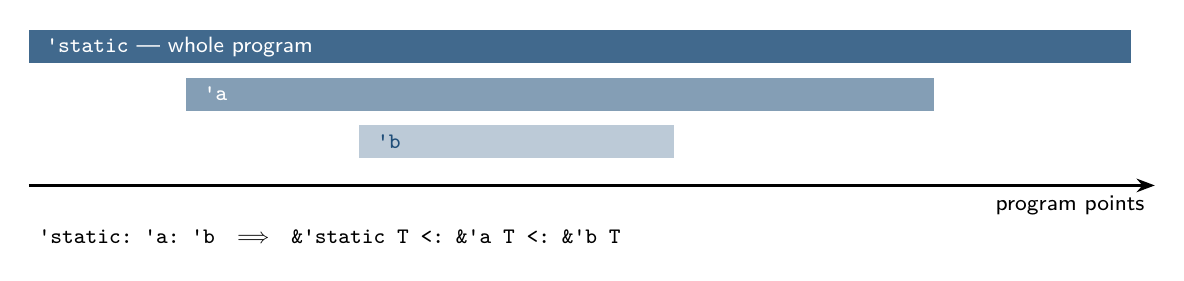
\begin{tikzpicture}[font=\sffamily\footnotesize]
  \fill[accent!85] (0,0) rectangle (14,0.42);\node[white,anchor=west] at (0.1,0.21) {\texttt{\textquotesingle static} --- whole program};
  \fill[accent!55] (2,-0.6) rectangle (11.5,-0.18);\node[white,anchor=west] at (2.1,-0.39) {\texttt{\textquotesingle a}};
  \fill[accent!30] (4.2,-1.2) rectangle (8.2,-0.78);\node[accent,anchor=west] at (4.3,-0.99) {\texttt{\textquotesingle b}};
  \draw[-{Stealth},thick] (0,-1.55) -- (14.3,-1.55) node[below left] {program points};
  \node[anchor=west] at (0,-2.2) {\texttt{\textquotesingle static: \textquotesingle a: \textquotesingle b}\quad $\Longrightarrow$\quad
   \texttt{\&\textquotesingle static T <: \&\textquotesingle a T <: \&\textquotesingle b T}};
\end{tikzpicture}
\caption{Outlives order on regions induces subtyping on shared references.}
\end{figure}

How a type constructor propagates this order is its \emph{variance} in each parameter:

\begin{center}
\begin{tabular}{@{}lcc@{}}
\toprule
\textbf{Type} & \textbf{in the lifetime} & \textbf{in \rs{T}}\\\midrule
\rs{&'a T} & covariant & covariant\\
\rs{&'a mut T} & covariant & \textbf{invariant}\\
\rs{Box<T>}, \rs{Vec<T>}, \rs{Option<T>} & --- & covariant\\
\rs{Cell<T>}, \rs{RefCell<T>}, \rs{UnsafeCell<T>} & --- & \textbf{invariant}\\
\rs{*const T} / \rs{*mut T} & --- & covariant / \textbf{invariant}\\
\rs{fn(T) -> U} & --- & \textbf{contravariant} in \rs{T}, covariant in \rs{U}\\
\rs{dyn Trait + 'a} & covariant & (trait's own parameters: invariant)\\
\bottomrule
\end{tabular}
\end{center}

\ok{ok_13_covariance}{Covariance: \texttt{\&\textquotesingle static str} shrinks to fit}
\ok{ok_17_box_covariance}{Covariance carries through \texttt{Box}}

Invariance is the safety net for \emph{writes}. If \rs{&mut &'a str} were covariant you could overwrite a long-lived
slot with a short-lived reference through a view that has forgotten the real lifetime:

\fail{fail_13_invariance}{\texttt{\&mut T} is invariant in \texttt{T}}
\diag{fail_13_invariance}

The same holds for interior mutability:

\fail{fail_17_cell_invariance}{\texttt{Cell<T>} is invariant in \texttt{T}}
\diag{fail_17_cell_invariance}

\textit{For the type-theoretically inclined:} the lifetimes form a preorder under \emph{outlives}; each type constructor
is a (co-, contra- or non-variant) functor on it. \rs{&mut T} places \rs{T} in both a read (covariant) and a write
(contravariant) position, and the two together force invariance. \st\ is the greatest element of the order.

% ================= 5 =================
\section{The anonymous lifetime \us}
\label{sec:underscore}

\subsection{What it means, precisely}

\us\ is \emph{not a lifetime name}: it cannot be referred to twice. Every occurrence introduces its own, independent
lifetime, and \emph{what that lifetime is} depends on where it appears:

\begin{longtable}{@{}p{3.7cm}p{5.5cm}p{6.2cm}@{}}
\toprule
\textbf{Position} & \textbf{Meaning of \us} & \textbf{Example}\\\midrule\endhead
Function \emph{parameter} type & A fresh lifetime parameter, identical to eliding it & \rs{x: &'_ str}, \rs{r: Ref<'_, T>}\\
Function \emph{return} type & Whichever input lifetime elision rules 2/3 select; E0106 if none & \rs{-> Iter<'_, T>}\\
\rs{impl} header & A fresh parameter, unnameable in the body & \rs{impl Display for Parser<'_>}\\
After \rs{+} on \rs{dyn}/\rs{impl} in a signature & The same elision choice as the return type & \rs{Box<dyn Fn() + '_>}, \rs{impl Iterator + '_}\\
Type in a \emph{body} (\rs{let}, turbofish) & An inference variable & \rs{let g: MutexGuard<'_, T> = ..}\\
Struct/enum field & \emph{Not allowed} (E0106) & \rs{struct S { r: &'_ str }}\\
\bottomrule
\end{longtable}

\begin{keyidea}
Read \us\ as ``a lifetime exists here, I don't need to name it''. Two occurrences are \textbf{never} forced to be equal:
\rs{fn f(a: &'_ str, b: &'_ str)} is \rs{fn f<'x, 'y>(a: &'x str, b: &'y str)}, not \rs{fn f<'a>(a: &'a str, b: &'a str)}.
\end{keyidea}

\subsection{Job 1 --- make hidden lifetime parameters visible}

Many std types carry a lifetime (\rs{Chars<'a>}, \rs{Ref<'b, T>}, \rs{fmt::Formatter<'_>}\dots). You may omit it,
but then a borrow is hidden in the signature. The lint \rs{elided_lifetimes_in_paths} (part of \rs{rust_2018_idioms})
flags it, and \us\ is the fix:

\ok{ok_04_underscore_return}{\texttt{SplitWhitespace<\textquotesingle\_>} vs.\ the hidden form}
\diag{ok_04_underscore_return}

\subsection{Job 2 --- impl headers, and when you need a real name instead}

\rs{impl Display for Parser<'_>} is the same as \rs{impl<'a> Display for Parser<'a>}; prefer the short form whenever the
body never mentions the lifetime (see \texttt{Display for Parser} in Listing~\ref{lst:parsersrc} and the
\rs{Formatter<'_>} parameter). As soon as you must \emph{refer} to it, e.g.\ to return \rs{Option<&'src str>}, you need a
name, and this is the dividing line between \us\ and a named lifetime. \rs{impl Parser<'_> { fn next_word(&mut self) -> Option<&'src str> }} cannot be written.

\subsection{Job 3 --- opting trait objects and \texorpdfstring{\texttt{impl Trait}}{impl Trait} into borrowing}

This is the use case that is least often explained. A trait object in a signature has a hidden lifetime bound, and for
\rs{Box<dyn ..>} the default is \st\ (Section~\ref{sec:defaults}). To let it borrow from a parameter, say so with \us:

\ok{ok_05_dyn_underscore}{\texttt{Box<dyn Fn(\&str) -> String + \textquotesingle\_>}}
\fail{fail_05_dyn_static}{Without \texttt{+ \textquotesingle\_} the closure must be \texttt{\textquotesingle static}}
\diag{fail_05_dyn_static}

Note that the compiler itself suggests \us. The same applies to \rs{impl Trait} in return position. In edition 2021 an
opaque type captures \emph{type} parameters but \emph{not} the lifetime of an elided reference argument unless you say so:

\ok{ok_06_rpit}{\texttt{impl Iterator + \textquotesingle\_}}
\fail{fail_06_rpit}{Edition 2021: the hidden type captures a lifetime that is not in the bounds}\label{lst:rpitfail}
\diag{fail_06_rpit}

\begin{pitfall}[Edition note]
Rust~2024 (stable since 1.85) changes return-position \rs{impl Trait} to capture \emph{all} in-scope lifetimes by default, so
Listing~\ref{lst:rpitfail} compiles there, and \rs{+ use<..>} (precise capturing, 1.82) lets you opt \emph{out}. I
verified the 2021 behaviour above with rustc 1.75; the 2024 statement is from my own knowledge of the edition, was not
checked by this document's build, and is worth confirming on your toolchain.
\end{pitfall}

\subsection{What \us\ cannot do}

\us\ does not resolve ambiguity. When elision has nothing to choose, writing \us\ in the output changes nothing:

\fail{fail_04_ambiguous}{\texttt{\textquotesingle\_} does not make an ambiguous signature legal}\label{lst:ambig}
\diag{fail_04_ambiguous}

It also does not mean ``infer it from the body''. Signature lifetimes are \emph{never} inferred from the body; only
body-level types (\rs{let x: Ref<'_, T>}) use \us\ as an inference placeholder.

\begin{tcolorbox}[enhanced,colback=white,colframe=accent!60,boxrule=0.4pt,arc=2pt,left=6pt,right=6pt,top=4pt,bottom=4pt,
  title={\sffamily\bfseries\small Checklist: which of \texttt{\textquotesingle a}, \texttt{\textquotesingle\_}, or nothing?},
  fonttitle=\sffamily\bfseries\small,colbacktitle=accent!10,coltitle=accent]
\begin{enumerate}[leftmargin=1.5em]
\item The lifetime appears once and I never mention it again $\Rightarrow$ \us\ (or elide it).
\item I need to tie two positions together (two inputs, or an input and the output) $\Rightarrow$ a \emph{named} lifetime.
\item I want the output to follow the \rs{&self} borrow $\Rightarrow$ elide, or write \us.
\item I want the output to follow a \emph{field's} lifetime rather than \rs{&self} $\Rightarrow$ name the struct's parameter.
\item A trait object/\rs{impl Trait} in a return type should borrow from an argument $\Rightarrow$ add \rs{+ '_} or \rs{+ 'a}.
\end{enumerate}
\end{tcolorbox}

% ================= 6 =================
\section{The \st\ lifetime}
\label{sec:static}

\subsection{Two meanings that are constantly conflated}

\begin{center}
\begin{tabular}{@{}p{3.4cm}p{5.2cm}p{6.1cm}@{}}
\toprule
\textbf{Form} & \textbf{What it is} & \textbf{What it says}\\\midrule
\rs{&'static T} & a \emph{reference type} & the pointee is valid for the remainder of the program (string literals, \rs{static} items, leaked allocations)\\\addlinespace
\rs{T: 'static} & a \emph{bound} on a type & every lifetime inside \rs{T} is \rs{'static}, i.e.\ \rs{T} contains no borrow that can expire. Owning types satisfy it\\
\bottomrule
\end{tabular}
\end{center}

Formally, \rs{&'a U: 'static} holds iff \rs{'a} is \rs{'static} (and \rs{U: 'static}); \rs{Foo<'a>: 'static} holds iff
\rs{'a} is \rs{'static}; a concrete type with no lifetime parameter anywhere inside it (such as \rs{String}) satisfies the bound unconditionally.

\begin{figure}[h]
\centering
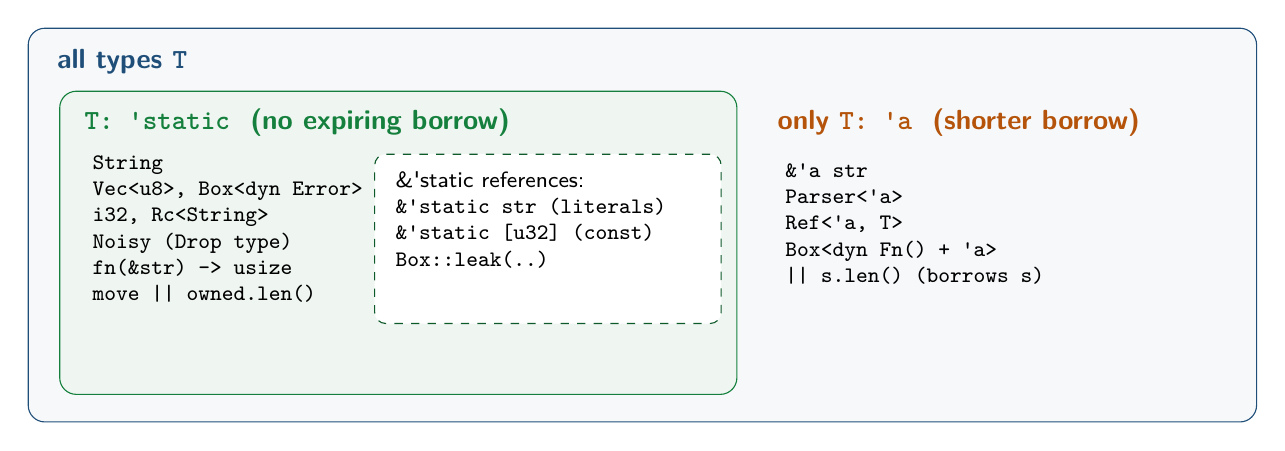
\begin{tikzpicture}[font=\sffamily\small]
  \node[draw=accent,rounded corners=6pt,fill=accent!4,minimum width=15.6cm,minimum height=5.0cm,anchor=north west] at (0,0) {};
  \node[anchor=north west,font=\sffamily\bfseries,text=accent] at (0.25,-0.15) {all types \texttt{T}};
  % inner set
  \node[draw=okgreen,rounded corners=6pt,fill=okgreen!7,minimum width=8.6cm,minimum height=3.85cm,anchor=north west] at (0.4,-0.8) {};
  \node[anchor=north west,font=\sffamily\bfseries,text=okgreen] at (0.6,-0.9) {\texttt{T: \textquotesingle static}\ \ (no expiring borrow)};
  \node[anchor=north west,align=left,font=\ttfamily\footnotesize] at (0.7,-1.5)
     {String\\Vec<u8>, Box<dyn Error>\\i32, Rc<String>\\Noisy (Drop type)\\fn(\&str) -> usize\\move || owned.len()};
  \node[draw=okgreen!70!black,dashed,rounded corners=4pt,fill=white,minimum width=4.4cm,minimum height=2.15cm,anchor=north west] at (4.4,-1.6) {};
  \node[anchor=north west,align=left,font=\ttfamily\footnotesize] at (4.55,-1.7)
     {\textsf{\&\textquotesingle static references:}\\\&\textquotesingle static str (literals)\\\&\textquotesingle static [u32] (const)\\Box::leak(..)};
  % outer-only
  \node[anchor=north west,align=left,font=\sffamily\bfseries,text=accent2] at (9.4,-0.9) {only \texttt{T: \textquotesingle a}\ \ (shorter borrow)};
  \node[anchor=north west,align=left,font=\ttfamily\footnotesize] at (9.5,-1.6)
     {\&\textquotesingle a str\\Parser<\textquotesingle a>\\Ref<\textquotesingle a, T>\\Box<dyn Fn() + \textquotesingle a>\\|| s.len()   (borrows s)};
\end{tikzpicture}
\caption{\texttt{T: \textquotesingle static} is a property of the \emph{type}; \texttt{\&\textquotesingle static T} is a small subset of it.}\label{fig:staticsets}
\end{figure}

\subsection{Where \refst\ references come from}

\ok{ok_07_static_sources}{Four sources of \texttt{\&\textquotesingle static}}
\runout{ok_07_static_sources}

\begin{itemize}
\item \textbf{Literals} live in the binary's read-only data. \rs{static} and \rs{const} items of reference type get \st\ by the item default rule.
\item \textbf{Constant promotion}: \rs{&42} or \rs{&[1, 2, 3]} in a function body is promoted to a static when the expression is constant and has no destructor or interior mutability. \rs{&String::new()} is \emph{not} promoted.
\item \textbf{Leaking}: \rs{Box::leak} returns \rs{&'a mut T} for any \rs{'a} you ask for, including \st. It is a deliberate memory leak: fine for process-lifetime singletons and interned strings, a bug when done per request.
\item \textbf{Globals} (\rs{static} + \rs{OnceLock}/\rs{LazyLock}) hand out \st\ references to lazily initialised data.
\end{itemize}

\subsection{\Tst\ does \emph{not} mean ``lives forever''}

The bound constrains the \emph{type}, not the \emph{value's} lifetime. A value of a \rs{'static} type can be created and dropped in
the same statement:

\ok{ok_08_static_bound}{A \texttt{\textquotesingle static} type that is dropped immediately}\label{lst:noisy}
\runout{ok_08_static_bound}
\fail{fail_08_static_bound}{Only a \emph{borrow} of a local fails the bound}
\diag{fail_08_static_bound}

So the practical test is ``does the type contain a borrow that can expire?'' (every ``yes'' row compiles in \texttt{ok\_15}; every ``no'' row is rejected in \texttt{fail\_15}):

\begin{center}
\begin{tabular}{@{}llp{6.4cm}@{}}
\toprule
\textbf{Type / value} & \rs{: 'static}? & \textbf{Why}\\\midrule
\rs{String}, \rs{Vec<String>}, \rs{i32} & \textcolor{okgreen}{yes} & owns all its data\\
\rs{&'static str} & \textcolor{okgreen}{yes} & the only lifetime inside is \st\\
\rs{Rc<String>} & \textcolor{okgreen}{yes} & iff the contents are\\
\rs{Box<dyn Error>} & \textcolor{okgreen}{yes} & default object bound is \st\\
\rs{fn(&str)}, fn items & \textcolor{okgreen}{yes} & no captured state\\
\rs{move} closure owning a \rs{String} & \textcolor{okgreen}{yes} & captures by value\\\addlinespace
\rs{&'a str} (local \rs{'a}) & \textcolor{badred}{no} & short borrow inside\\
\rs{Parser<'a>} & \textcolor{badred}{no} & lifetime parameter is not \st\\
non-\rs{move} closure using a local & \textcolor{badred}{no} & captures a borrow\\
\bottomrule
\end{tabular}
\end{center}

\subsection{Why APIs ask for \Tst}

{\sffamily\bfseries Threads and tasks.} \rs{thread::spawn} (and async runtimes' \rs{spawn}) hand the closure to something that
may outlive the caller's stack frame, so it cannot contain borrows of that frame. Either move ownership in, or use
\emph{scoped} threads, which are joined before the borrowed data can die and therefore need no \st:

\ok{ok_09_threads}{Own it, or borrow it with \texttt{thread::scope}}
\runout{ok_09_threads}
\fail{fail_09_spawn_borrow}{Borrowing a local into \texttt{thread::spawn}}
\diag{fail_09_spawn_borrow}

{\sffamily\bfseries \texttt{Any} and downcasting.} \rs{Any} requires \st\ because \rs{TypeId} is computed \emph{after}
lifetimes are erased: \rs{&'a T} and \rs{&'b T} would be indistinguishable, and downcasting could then forge lifetimes.

{\sffamily\bfseries Trait objects stored for a long time.} \rs{Box<dyn Error>}, callbacks in registries and \rs{Arc<dyn Trait>}
fields all default to \st.

{\sffamily\bfseries Generic propagation.} If your generic function calls any of the above, the bound must appear on \emph{your}
\rs{T} too:

\fail{fail_14_E0310}{E0310: the bound has to be written on the generic parameter}
\diag{fail_14_E0310}
\ok{ok_14_E0310_fixed}{Adding \texttt{+ \textquotesingle static} fixes it}

\subsection{Defaults for trait-object lifetime bounds}
\label{sec:defaults}

When you write \rs{dyn Trait} without a lifetime bound, the compiler picks one from the surrounding type:

\begin{center}
\begin{tabular}{@{}p{4.8cm}p{5.2cm}p{4.7cm}@{}}
\toprule
\textbf{You write} & \textbf{It means} & \textbf{Rule}\\\midrule
\rs{Box<dyn T>} & \rs{Box<dyn T + 'static>} & container has no lifetime\\
\rs{Rc<dyn T>}, \rs{Arc<dyn T>} & \rs{... dyn T + 'static} & same\\
\rs{&'a dyn T} & \rs{&'a (dyn T + 'a)} & bounded by the reference\\
\rs{&'a mut dyn T} & \rs{&'a mut (dyn T + 'a)} & same\\
\rs{Ref<'a, dyn T>} & \rs{Ref<'a, dyn T + 'a>} & parameter has \rs{T: 'a}\\
\rs{trait T: 'x}, then \rs{dyn T} & \rs{dyn T + 'x} & trait's own bound\\
\rs{dyn T} inside a fn \emph{body} & inferred & expression context\\
\bottomrule
\end{tabular}
\end{center}

This asymmetry is the root of the infamous ``\emph{returning this value requires that \rs{'1} must outlive \rs{'static}}'' error.
The complete program below names the bound; deleting \rs{+ 'a} reproduces the error (second listing).

\ok{ok_10_object_defaults}{Name the bound where the object must borrow}
\runout{ok_10_object_defaults}
\fail{fail_10_boxed_static}{Plain \texttt{Box<dyn Shape>} silently means \texttt{+ \textquotesingle static}}
\diag{fail_10_boxed_static}

The same trap hides behind \rs{?} and \rs{Box<dyn Error>}: an error type that \emph{borrows} from its input cannot be
converted into the default \rs{Box<dyn Error>}.

\ok{ok_11_error_box}{\texttt{Box<dyn Error + \textquotesingle\_>} (often better still: own the data in the error)}
\runout{ok_11_error_box}
\fail{fail_11_error_box}{Default \texttt{Box<dyn Error>} demands \texttt{\textquotesingle static}}
\diag{fail_11_error_box}

\subsection{Myths and anti-patterns}

\begin{longtable}{@{}p{5.6cm}p{9.8cm}@{}}
\toprule
\textbf{Myth / habit} & \textbf{Reality}\\\midrule\endhead
``\rs{T: 'static} means the value lives for the whole program.'' & It restricts the \emph{type}. A \rs{String} local to one function is \rs{'static}; it is dropped normally (Listing~\ref{lst:noisy}).\\
``The compiler says \st\ so I'll add \rs{&'static} to the parameter.'' & You have just forced every caller to supply literals or leaked data. Usually the error means a trait-object or spawn bound (see above); fix \emph{that}.\\
``Leak it; it's only a small \rs{String}.'' & \rs{Box::leak} per call is an unbounded memory leak. Acceptable for one-time configuration, interned names, and test fixtures only.\\
``\rs{struct Cfg { name: &'static str }} is flexible.'' & It accepts only literals and leaked strings. Prefer \rs{String}, \rs{Arc<str>}, a lifetime parameter \rs{Cfg<'a>}, or \rs{Cow<'static, str>} when most values are literals.\\
``\rs{&'static} and \rs{T: 'static} are the same thing.'' & One is a reference whose pointee lives forever, the other a closure under owned data (Figure~\ref{fig:staticsets}).\\
\bottomrule
\end{longtable}

\begin{keyidea}[A decision ladder for ``I need this to be \texttt{\textquotesingle static}'']
\begin{enumerate}[leftmargin=1.5em]
\item \textbf{Own it}: clone, \rs{String}, \rs{Vec}, or share with \rs{Arc}.
\item \textbf{Scope it}: \rs{thread::scope}, a borrowing struct \rs{Foo<'a>}, a bound like \rs{dyn Trait + 'a}.
\item \textbf{Mix}: \rs{Cow<'a, str>} or \rs{Cow<'static, str>}.
\item \textbf{Leak or global}: \rs{Box::leak}, \rs{OnceLock}, \rs{LazyLock} --- only for genuine process-lifetime data.
\end{enumerate}
\end{keyidea}

% ================= 7 =================
\section{Higher-ranked bounds: \texorpdfstring{\texttt{for<\textquotesingle a>}}{for<'a>}}
\label{sec:hrtb}

A bound such as \rs{F: Fn(&str) -> &str} is sugar for \rs{F: for<'a> Fn(&'a str) -> &'a str}: ``works for \emph{every}
lifetime'', not for one lifetime fixed by the caller. This is what lets \rs{f} be called on a string created inside the
function. You write \rs{for<'a>} explicitly only when the lifetime appears somewhere the sugar does not reach, for example on a
reference to a generic parameter:

\ok{ok_12_hrtb}{Explicit \texttt{for<\textquotesingle a>} on \texttt{\&\textquotesingle a C}}
\runout{ok_12_hrtb}

% ================= 8 =================
\section{Error catalogue}

\begin{longtable}{@{}p{1.5cm}p{4.0cm}p{4.9cm}p{4.4cm}@{}}
\toprule
\textbf{Code} & \textbf{Message} & \textbf{Usually means} & \textbf{Typical fix}\\\midrule\endhead
E0106 & missing lifetime specifier & Elision has no unique answer, or a field has no lifetime & Name a lifetime; add \rs{'a} to the struct\\
E0261 & use of undeclared lifetime name & \rs{'a} used but not declared in \rs{<..>} & Declare \rs{<'a>} on the fn/impl/struct\\
E0597 & \rs{x} does not live long enough & A reference outlives its referent; also fires for \rs{T: 'static} arguments & Shorten the use, move/clone the value, or restructure scopes\\
E0499 & cannot borrow as mutable more than once & Often an elided \rs{&mut self} lifetime pinning results & Return the struct's own lifetime (Listing~\ref{lst:parsersrc})\\
E0502 & mutable borrow while immutably borrowed & A shared borrow is still live at the conflicting access & Reorder, end the borrow earlier, or clone\\
E0505 & move out while borrowed & Moving a value that a live borrow points to & Borrow after the move or clone\\
E0373 & closure may outlive the current function & Non-\rs{move} closure given to \rs{spawn}-like API & \rs{move}, or \rs{thread::scope}\\
E0310 & parameter type \rs{T} may not live long enough & Generic code needs \rs{T: 'static} (or \rs{T: 'a}) & Add the bound on the parameter\\
E0700 & hidden type captures lifetime not in bounds & \rs{impl Trait} in edition 2021 hides a borrow & Add \rs{+ '_} / \rs{+ 'a}; or edition 2024\\
E0716 & temporary value dropped while borrowed & Borrowing a temporary beyond its statement & Bind it to a \rs{let}\\
E0521 & borrowed data escapes outside of function & A short borrow flows into a longer-lived place & Own the data, or add an explicit lifetime relation\\
{\scriptsize(none)} & lifetime may not live long enough & Region constraint violated between two signature lifetimes; often \rs{'1: 'static} from a default object bound & Compare the lifetimes the message names; add \rs{'_}/\rs{'a} bounds\\
\bottomrule
\end{longtable}

{\small Codes E0106, E0261, E0597, E0499, E0502, E0373, E0310 and E0700 appear in programs verified in this document. E0505, E0716 and E0521 are listed from general knowledge of the compiler.}

% ================= 9 =================
\clearpage
\section{Quick reference}

\begin{longtable}{@{}p{6.7cm}p{8.7cm}@{}}
\toprule
\textbf{I want to\dots} & \textbf{Write}\\\midrule\endhead
return a reference derived from the single input & elide: \rs{fn f(x: &T) -> &U}\\
return a view/iterator over \rs{&self} & \rs{-> Iter<'_, T>} or \rs{-> impl Iterator<Item = &T> + '_}\\
return data from a struct field's referent, not the \rs{&mut self} borrow & \rs{impl<'a> S<'a> { fn f(&mut self) -> &'a T }}\\
tie two parameters to the result & \rs{fn f<'a>(x: &'a T, y: &'a T) -> &'a T}\\
implement a trait for a borrowing type & \rs{impl Trait for Wrapper<'_>} (name it only if used)\\
return a closure/trait object that captures an argument & \rs{Box<dyn Fn(..) -> .. + '_>}\\
store a trait object in a long-lived struct & \rs{Box<dyn Trait>} (\st) or \rs{struct S<'a> { b: Box<dyn Trait + 'a> }}\\
run a closure on another thread with borrowed data & \rs{thread::scope(|s| { s.spawn(|| ..); })}\\
make generic code spawnable & \rs{T: Send + 'static}\\
return an error that borrows its input & \rs{Result<_, Box<dyn Error + '_>>}, or own the data in the error\\
accept a callback that handles any borrow & \rs{F: for<'a> Fn(&'a str) -> &'a str} (or \rs{Fn(&str) -> &str})\\
\bottomrule
\end{longtable}

\subsection*{Ten rules that cover most real code}
\begin{enumerate}
\item A lifetime is a region of program points, not a duration; annotations never extend one.
\item Only signatures need lifetimes; bodies are inferred.
\item Elision picks the single input, else \rs{&self}, else fails.
\item The \rs{&mut self} borrow and a struct's own lifetime are different lifetimes; return the one you mean.
\item \us\ = ``a lifetime I don't need to name''; never ``the same as the other one''.
\item \us\ after \rs{+} on a trait object or \rs{impl Trait} opts it into borrowing from the elided input.
\item \rs{&mut T} and \rs{Cell<T>} are invariant in \rs{T}; shared references are covariant.
\item \rs{&'static T} is a reference; \rs{T: 'static} is a bound that owned types satisfy.
\item \rs{Box<dyn Trait>} means \rs{+ 'static}; \rs{&'a dyn Trait} means \rs{+ 'a}.
\item When tempted to add \st, first try owning, scoping, or \rs{Cow}.
\end{enumerate}

% ================= Appendix =================
\appendix
\clearpage
\section{Verification log}

Each program was compiled with \texttt{rustc 1.75.0 --edition 2021} (Ubuntu package). ``Expected'' follows the file prefix:
\texttt{ok\_} must compile, \texttt{fail\_} must be rejected. The last column is the first diagnostic of the real run.

{\renewcommand{\arraystretch}{1.05}\begin{longtable}{@{}p{4.8cm}p{1.4cm}p{1.5cm}p{7.0cm}@{}}
\toprule \textbf{Program} & \textbf{Expected} & \textbf{Result} & \textbf{First diagnostic} \\\midrule\endhead
\texttt{\detokenize{fail_01_dangling.rs}} & rejected & \textcolor{okgreen}{pass} & {\scriptsize \texttt{\detokenize{error[E0597]: `inner` does not live long enough}}}\\
\texttt{\detokenize{ok_01_longest.rs}} & compiles & \textcolor{okgreen}{pass} & {\scriptsize ---}\\
\texttt{\detokenize{fail_02_nll.rs}} & rejected & \textcolor{okgreen}{pass} & {\scriptsize \texttt{\detokenize{error[E0502]: cannot borrow `v` as mutable because it is also borrowed as immutable}}}\\
\texttt{\detokenize{ok_02_nll.rs}} & compiles & \textcolor{okgreen}{pass} & {\scriptsize ---}\\
\texttt{\detokenize{fail_03_elided_self.rs}} & rejected & \textcolor{okgreen}{pass} & {\scriptsize \texttt{\detokenize{error[E0499]: cannot borrow `p` as mutable more than once at a time}}}\\
\texttt{\detokenize{ok_03_parser.rs}} & compiles & \textcolor{okgreen}{pass} & {\scriptsize ---}\\
\texttt{\detokenize{fail_04_ambiguous.rs}} & rejected & \textcolor{okgreen}{pass} & {\scriptsize \texttt{\detokenize{error[E0106]: missing lifetime specifier  (+1 more)}}}\\
\texttt{\detokenize{ok_04_underscore_return.rs}} & compiles & \textcolor{okgreen}{pass} & {\scriptsize \texttt{\detokenize{warning: hidden lifetime parameters in types are deprecated}}}\\
\texttt{\detokenize{fail_05_dyn_static.rs}} & rejected & \textcolor{okgreen}{pass} & {\scriptsize \texttt{\detokenize{error: lifetime may not live long enough}}}\\
\texttt{\detokenize{ok_05_dyn_underscore.rs}} & compiles & \textcolor{okgreen}{pass} & {\scriptsize ---}\\
\texttt{\detokenize{fail_06_rpit.rs}} & rejected & \textcolor{okgreen}{pass} & {\scriptsize \texttt{\detokenize{error[E0700]: hidden type for `impl Iterator<Item = char>` captures lifetime that doe...}}}\\
\texttt{\detokenize{ok_06_rpit.rs}} & compiles & \textcolor{okgreen}{pass} & {\scriptsize ---}\\
\texttt{\detokenize{ok_07_static_sources.rs}} & compiles & \textcolor{okgreen}{pass} & {\scriptsize ---}\\
\texttt{\detokenize{fail_08_static_bound.rs}} & rejected & \textcolor{okgreen}{pass} & {\scriptsize \texttt{\detokenize{error[E0597]: `local` does not live long enough}}}\\
\texttt{\detokenize{ok_08_static_bound.rs}} & compiles & \textcolor{okgreen}{pass} & {\scriptsize ---}\\
\texttt{\detokenize{fail_09_spawn_borrow.rs}} & rejected & \textcolor{okgreen}{pass} & {\scriptsize \texttt{\detokenize{error[E0373]: closure may outlive the current function, but it borrows `data`, which ...}}}\\
\texttt{\detokenize{ok_09_threads.rs}} & compiles & \textcolor{okgreen}{pass} & {\scriptsize ---}\\
\texttt{\detokenize{fail_10_boxed_static.rs}} & rejected & \textcolor{okgreen}{pass} & {\scriptsize \texttt{\detokenize{error: lifetime may not live long enough}}}\\
\texttt{\detokenize{ok_10_object_defaults.rs}} & compiles & \textcolor{okgreen}{pass} & {\scriptsize ---}\\
\texttt{\detokenize{fail_11_error_box.rs}} & rejected & \textcolor{okgreen}{pass} & {\scriptsize \texttt{\detokenize{error: lifetime may not live long enough}}}\\
\texttt{\detokenize{ok_11_error_box.rs}} & compiles & \textcolor{okgreen}{pass} & {\scriptsize \texttt{\detokenize{error[E0597]: `text` does not live long enough}}}\\
\texttt{\detokenize{ok_12_hrtb.rs}} & compiles & \textcolor{okgreen}{pass} & {\scriptsize ---}\\
\texttt{\detokenize{fail_13_invariance.rs}} & rejected & \textcolor{okgreen}{pass} & {\scriptsize \texttt{\detokenize{error[E0597]: `local` does not live long enough}}}\\
\texttt{\detokenize{ok_13_covariance.rs}} & compiles & \textcolor{okgreen}{pass} & {\scriptsize ---}\\
\texttt{\detokenize{fail_14_E0310.rs}} & rejected & \textcolor{okgreen}{pass} & {\scriptsize \texttt{\detokenize{error[E0310]: the parameter type `T` may not live long enough}}}\\
\texttt{\detokenize{ok_14_E0310_fixed.rs}} & compiles & \textcolor{okgreen}{pass} & {\scriptsize ---}\\
\texttt{\detokenize{fail_15_static_table_no.rs}} & rejected & \textcolor{okgreen}{pass} & {\scriptsize \texttt{\detokenize{error[E0597]: `s` does not live long enough  (+2 more)}}}\\
\texttt{\detokenize{ok_15_static_table.rs}} & compiles & \textcolor{okgreen}{pass} & {\scriptsize ---}\\
\texttt{\detokenize{fail_16_struct_field_elided.rs}} & rejected & \textcolor{okgreen}{pass} & {\scriptsize \texttt{\detokenize{error[E0106]: missing lifetime specifier  (+2 more)}}}\\
\texttt{\detokenize{fail_17_cell_invariance.rs}} & rejected & \textcolor{okgreen}{pass} & {\scriptsize \texttt{\detokenize{error[E0597]: `local` does not live long enough}}}\\
\texttt{\detokenize{ok_17_box_covariance.rs}} & compiles & \textcolor{okgreen}{pass} & {\scriptsize ---}\\
\texttt{\detokenize{fail_18_elision_cases.rs}} & rejected & \textcolor{okgreen}{pass} & {\scriptsize \texttt{\detokenize{error[E0106]: missing lifetime specifier  (+1 more)}}}\\
\texttt{\detokenize{ok_18_elision_fixes.rs}} & compiles & \textcolor{okgreen}{pass} & {\scriptsize ---}\\
\texttt{\detokenize{fail_19_struct_single_ref.rs}} & rejected & \textcolor{okgreen}{pass} & {\scriptsize \texttt{\detokenize{error[E0106]: missing lifetime specifier}}}\\
\texttt{\detokenize{ok_19_struct_fixes.rs}} & compiles & \textcolor{okgreen}{pass} & {\scriptsize ---}\\
\texttt{\detokenize{fail_20_static_field_local.rs}} & rejected & \textcolor{okgreen}{pass} & {\scriptsize \texttt{\detokenize{error[E0597]: `text` does not live long enough}}}\\
\texttt{\detokenize{fail_21_rule_first.rs}} & rejected & \textcolor{okgreen}{pass} & {\scriptsize \texttt{\detokenize{error: lifetime may not live long enough  (+1 more)}}}\\
\texttt{\detokenize{ok_21_lookup_explicit.rs}} & compiles & \textcolor{okgreen}{pass} & {\scriptsize ---}\\
\texttt{\detokenize{fail_22_rule_unify.rs}} & rejected & \textcolor{okgreen}{pass} & {\scriptsize \texttt{\detokenize{error[E0597]: `key` does not live long enough}}}\\
\texttt{\detokenize{fail_23_contract_v2.rs}} & rejected & \textcolor{okgreen}{pass} & {\scriptsize \texttt{\detokenize{error[E0597]: `short` does not live long enough}}}\\
\texttt{\detokenize{ok_23_contract_v1.rs}} & compiles & \textcolor{okgreen}{pass} & {\scriptsize ---}\\
\texttt{\detokenize{fail_24_trait_no_body.rs}} & rejected & \textcolor{okgreen}{pass} & {\scriptsize \texttt{\detokenize{error[E0106]: missing lifetime specifier}}}\\
\bottomrule\end{longtable}}


\section{Further reading}

Titles only; I could not open or check any of these while writing, so please confirm sections and current wording yourself:
\emph{The Rust Programming Language} (generic types, traits and lifetimes chapter); \emph{The Rust Reference}
(lifetime elision, trait object lifetime bounds, subtyping and variance); \emph{The Rustonomicon} (lifetimes, subtyping and variance,
higher-rank trait bounds); RFC~2094 (non-lexical lifetimes).

\end{document}
